% CENTRAL OBSERVABILITY VISUALS — REVIEW ADDENDUM (B1–B6)
% Companion to CENTRAL_OBSERVABILITY_REVIEW_ADDENDUM.md; same visual language
% as CENTRAL_OBSERVABILITY_VISUALS.tex. Compile: pdflatex (twice).
\documentclass[10pt]{article}
\usepackage[a4paper,landscape,margin=10mm]{geometry}
\usepackage[T1]{fontenc}
\usepackage[utf8]{inputenc}
\usepackage[sc]{mathpazo}
\usepackage{microtype}
\usepackage{tikz}
\usetikzlibrary{arrows.meta,positioning,fit,calc,backgrounds,shapes.geometric,shapes.multipart,decorations.pathreplacing,matrix}
\usepackage{xcolor}
\usepackage{colortbl}
\usepackage{array,booktabs}
\usepackage{adjustbox}
\usepackage{hyperref}
\hypersetup{hidelinks}
\pagestyle{empty}
\setlength{\parindent}{0pt}
\setlength{\tabcolsep}{4pt}
\renewcommand{\arraystretch}{1.15}

\definecolor{store}{HTML}{EAF0FF}
\definecolor{source}{HTML}{EAF8EC}
\definecolor{writer}{HTML}{FFF0EE}
\definecolor{reader}{HTML}{F6EDFA}
\definecolor{ci}{HTML}{FFF5E6}
\definecolor{external}{HTML}{F4F4F4}
\definecolor{risk}{HTML}{FFE3E3}
\definecolor{good}{HTML}{E2F5E7}
\definecolor{policy}{HTML}{E8F7F5}
\definecolor{ink}{HTML}{263238}
\definecolor{muted}{HTML}{607D8B}
\definecolor{red}{HTML}{B54A4A}
\definecolor{purple}{HTML}{7A4E9B}
\definecolor{orange}{HTML}{B56A24}
\definecolor{green}{HTML}{39784A}
\definecolor{blue}{HTML}{3F6FB5}

\tikzset{
  >=Latex,
  every node/.style={font=\small,text=ink},
  box/.style={draw=ink!65,rounded corners=2.5pt,fill=store,minimum height=11mm,minimum width=34mm,align=center,inner sep=4pt},
  sourcebox/.style={box,fill=source,draw=green!70},
  writerbox/.style={box,fill=writer,draw=red!70},
  readerbox/.style={box,fill=reader,draw=purple!70},
  cibox/.style={box,fill=ci,draw=orange!75},
  extbox/.style={box,fill=external,dashed},
  policybox/.style={box,fill=policy,draw=green!70},
  riskbox/.style={box,fill=risk,draw=red!80},
  goodbox/.style={box,fill=good,draw=green!75},
  tinybox/.style={draw=ink!55,rounded corners=2pt,fill=white,align=center,inner sep=3pt,font=\footnotesize},
  state/.style={draw=ink!65,rounded corners=6pt,fill=store,minimum width=28mm,minimum height=10mm,align=center},
  terminal/.style={state,fill=good,draw=green!75},
  badstate/.style={state,fill=risk,draw=red!80},
  arrow/.style={->,very thick,draw=ink!75},
  async/.style={->,thick,dashed,draw=purple},
  write/.style={->,very thick,draw=red},
  policyarr/.style={->,very thick,draw=green},
  effect/.style={->,very thick,draw=orange},
  fail/.style={->,very thick,dashed,draw=red},
  note/.style={draw=ink!30,rounded corners=2pt,fill=white,align=left,inner sep=5pt,font=\footnotesize,text width=70mm},
  pill/.style={draw=ink!45,rounded corners=7pt,fill=white,inner xsep=6pt,inner ysep=2pt,font=\footnotesize\bfseries},
  label/.style={font=\footnotesize,align=center,fill=white,inner sep=1.5pt},
}
\newcommand{\code}[1]{\texttt{\detokenize{#1}}}
\newcommand{\pagehead}[2]{%
  \begin{minipage}[t]{0.73\linewidth}
    {\Large\bfseries #1}\\[-1mm]
    {\small\color{muted}#2}
  \end{minipage}\hfill
  \begin{minipage}[t]{0.25\linewidth}\raggedleft
    {\footnotesize Central observability - review \textbf{addendum}}\\
    {\scriptsize companion to REVIEW\_ADDENDUM.md - 2026-07-06}
  \end{minipage}
  \vspace{3mm}\hrule\vspace{4mm}
}
\newcommand{\legend}{%
\tikz[baseline=-0.7ex]\node[sourcebox,minimum width=7mm,minimum height=4mm,inner sep=1pt]{}; sources\quad
\tikz[baseline=-0.7ex]\node[writerbox,minimum width=7mm,minimum height=4mm,inner sep=1pt]{}; writers\quad
\tikz[baseline=-0.7ex]\node[policybox,minimum width=7mm,minimum height=4mm,inner sep=1pt]{}; policy/contract\quad
\tikz[baseline=-0.7ex]\node[box,minimum width=7mm,minimum height=4mm,inner sep=1pt]{}; store\quad
\tikz[baseline=-0.7ex]\node[readerbox,minimum width=7mm,minimum height=4mm,inner sep=1pt]{}; readers\quad
\tikz[baseline=-0.7ex]\node[cibox,minimum width=7mm,minimum height=4mm,inner sep=1pt]{}; CI/automation\quad
\tikz[baseline=-0.7ex]\node[riskbox,minimum width=7mm,minimum height=4mm,inner sep=1pt]{}; correction/hazard
}

\begin{document}

% =====================================================================
% B1. INGEST STATE MACHINE
% =====================================================================
\pagehead{B1. Ingest protocol: disposition at begin, visibility by construction}
{C-2/C-3: the entity lock decides insert/duplicate/reproject/refuse \textbf{before} any kind row is staged; readers can only ever see the current batch.}
\legend\par\vspace{4mm}

\begin{adjustbox}{max width=\linewidth,max height=0.82\textheight,center}
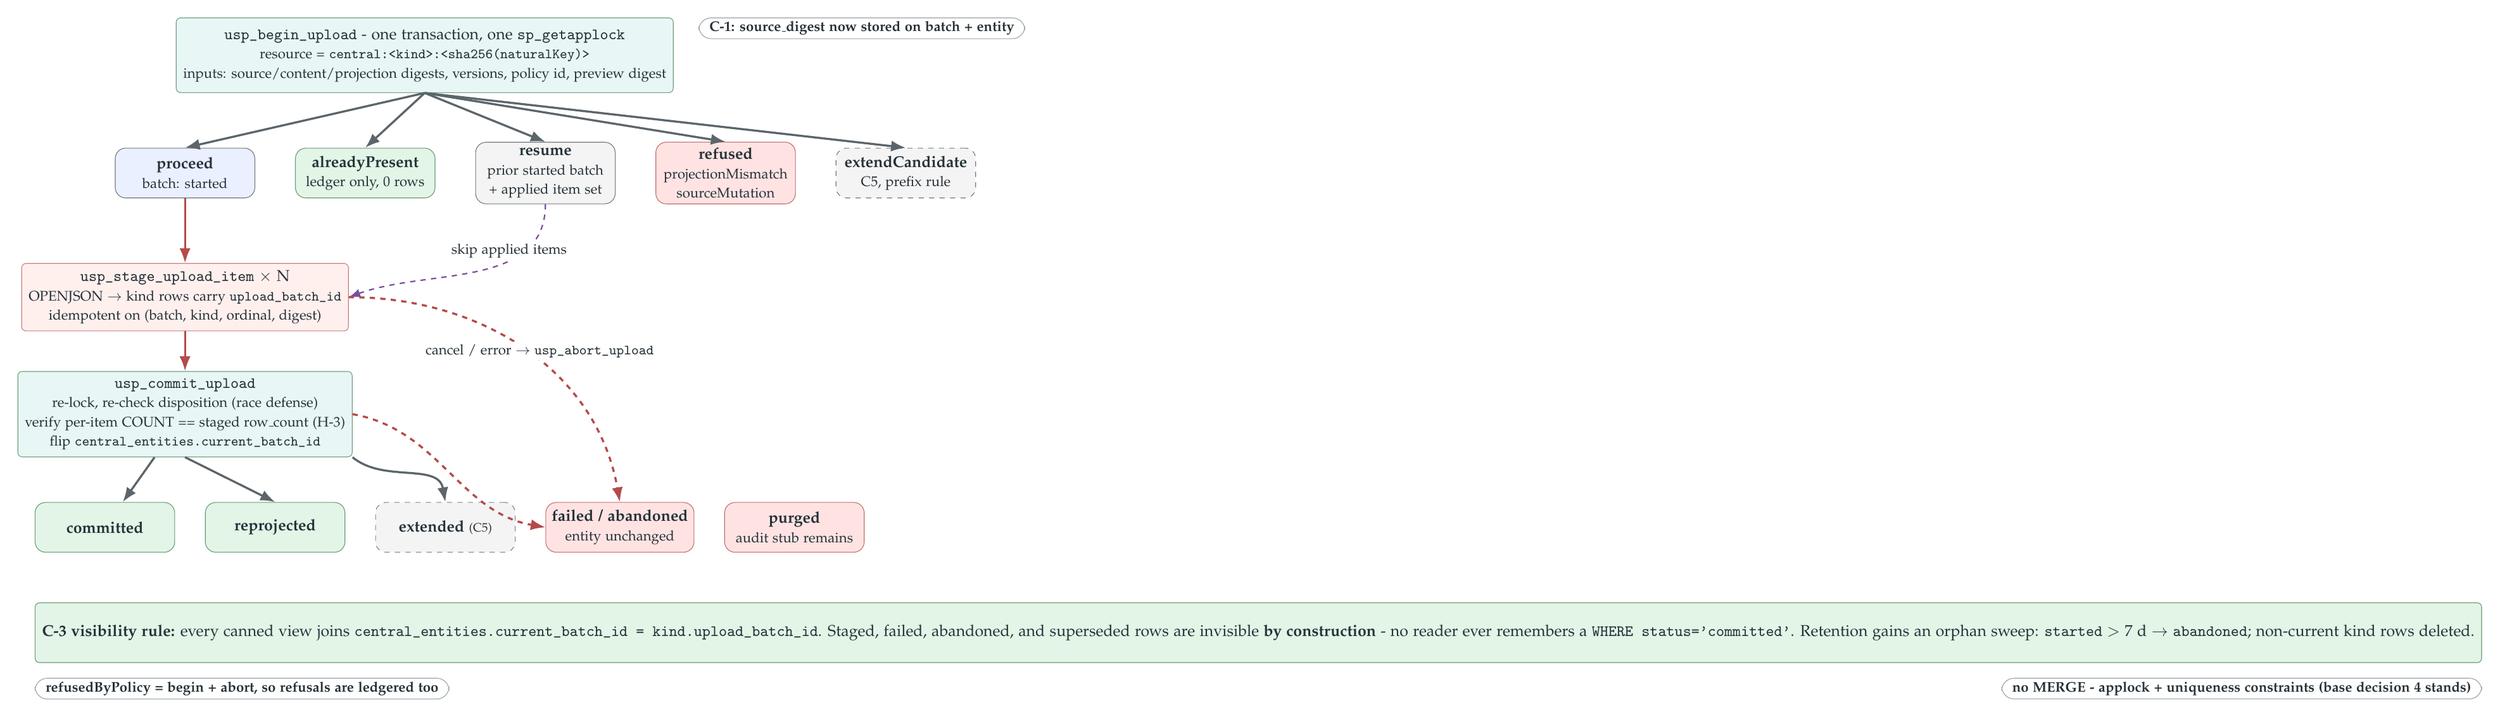
\begin{tikzpicture}[node distance=6mm and 7mm]

\node[policybox,minimum width=96mm,minimum height=15mm] (begin)
{\textbf{\code{usp_begin_upload}} - one transaction, one \code{sp_getapplock}\\\footnotesize resource = \code{central:<kind>:<sha256(naturalKey)>}\\\footnotesize inputs: source/content/projection digests, versions, policy id, preview digest};
\node[pill,right=5mm of begin.north east,anchor=north west] {C-1: source\_digest now stored on batch + entity};

% dispositions
\node[state,below left=11mm and 34mm of begin.south] (proceed) {\textbf{proceed}\\\footnotesize batch: started};
\node[terminal,right=8mm of proceed] (already) {\textbf{alreadyPresent}\\\footnotesize ledger only, 0 rows};
\node[state,right=8mm of already,fill=external] (resume) {\textbf{resume}\\\footnotesize prior started batch\\\footnotesize + applied item set};
\node[badstate,right=8mm of resume] (refused) {\textbf{refused}\\\footnotesize projectionMismatch\\\footnotesize sourceMutation};
\node[state,right=8mm of refused,fill=external,dashed] (extendc) {\textbf{extendCandidate}\\\footnotesize C5, prefix rule};
\foreach \d in {proceed,already,resume,refused,extendc}{\draw[arrow] (begin.south) -- (\d.north);}

% staging
\node[writerbox,minimum width=58mm,below=13mm of proceed] (stage)
{\textbf{\code{usp_stage_upload_item}} $\times$ N\\\footnotesize OPENJSON $\to$ kind rows carry \code{upload_batch_id}\\\footnotesize idempotent on (batch, kind, ordinal, digest)};
\draw[write] (proceed) -- (stage);
\draw[async] (resume.south) to[out=-90,in=20] node[label,above,pos=0.35]{skip applied items} (stage.east);

\node[policybox,minimum width=58mm,below=8mm of stage] (commit)
{\textbf{\code{usp_commit_upload}}\\\footnotesize re-lock, re-check disposition (race defense)\\\footnotesize verify per-item COUNT == staged row\_count (H-3)\\\footnotesize flip \code{central_entities.current_batch_id}};
\draw[write] (stage) -- (commit);

\node[terminal,below left=9mm and 2mm of commit.south] (committed) {\textbf{committed}};
\node[terminal,right=6mm of committed,fill=good] (reproj) {\textbf{reprojected}};
\node[terminal,right=6mm of reproj,fill=external,dashed,draw=ink!60] (extended) {\textbf{extended} \scriptsize(C5)};
\node[badstate,right=6mm of extended] (failed) {\textbf{failed / abandoned}\\\footnotesize entity unchanged};
\node[badstate,right=6mm of failed] (purged) {\textbf{purged}\\\footnotesize audit stub remains};
\draw[arrow] (commit) -- (committed);
\draw[arrow] (commit.south) -- (reproj.north);
\draw[arrow] (commit.south east) to[out=-40,in=100] (extended.north);
\draw[fail] (stage.east) to[out=0,in=100] node[label,above,pos=0.55]{cancel / error $\to$ \code{usp_abort_upload}} (failed.north);
\draw[fail] (commit.east) to[out=-10,in=170] (failed.west);

% visibility rule
\node[goodbox,minimum width=176mm,minimum height=12mm,below=10mm of committed.south west,anchor=north west] (vis)
{\textbf{C-3 visibility rule:} every canned view joins \code{central_entities.current_batch_id = kind.upload_batch_id}. Staged, failed, abandoned, and superseded rows are invisible \textbf{by construction} - no reader ever remembers a \code{WHERE status='committed'}. Retention gains an orphan sweep: \code{started} $>$ 7 d $\to$ \code{abandoned}; non-current kind rows deleted.};

\node[pill,below=3mm of vis.south west,anchor=north west] {refusedByPolicy = begin + abort, so refusals are ledgered too};
\node[pill,below=3mm of vis.south east,anchor=north east] {no MERGE - applock + uniqueness constraints (base decision 4 stands)};

\end{tikzpicture}
\end{adjustbox}

\newpage
% =====================================================================
% B2. DISPOSITION ALGEBRA / DIGEST POINTS
% =====================================================================
\pagehead{B2. The digest algebra: why \code{source_digest} must be persisted}
{C-1: \code{content_digest} is policy-filtered, so a policy change alone flips it. Without the pre-policy digest, a legitimate re-upload is indistinguishable from evidence mutation.}
\legend\par\vspace{4mm}

\begin{adjustbox}{max width=\linewidth,max height=0.82\textheight,center}
\begin{minipage}{270mm}

\begin{tikzpicture}[node distance=6mm and 9mm]
\node[sourcebox,minimum width=44mm] (src) {\textbf{source artifacts}\\\footnotesize manifest + segments /\\\footnotesize result.json + run files};
\node[tinybox,below=2.5mm of src] (sd) {\code{source_digest} - pre-policy inventory};
\node[policybox,minimum width=40mm,right=of src] (up) {\textbf{upload policy}\\\footnotesize keep / digest / drop\\\footnotesize on \{cls, handling\}};
\node[sourcebox,minimum width=42mm,right=of up] (content) {\textbf{filtered content}};
\node[tinybox,below=2.5mm of content] (cd) {\code{content_digest}};
\node[policybox,minimum width=40mm,right=of content] (proj) {\textbf{row projection}\\\footnotesize generated DTOs};
\node[sourcebox,minimum width=40mm,right=of proj] (rows) {\textbf{row stream}};
\node[tinybox,below=2.5mm of rows] (pd) {\code{projection_digest}};
\node[tinybox,right=8mm of pd] (prd) {\code{preview_digest} = sha256(canonical preview) (C-15)};
\draw[arrow] (src) -- (up);
\draw[policyarr] (up) -- (content);
\draw[arrow] (content) -- (proj);
\draw[policyarr] (proj) -- (rows);
\end{tikzpicture}

\vspace{5mm}
\begin{tabular}{p{34mm}p{50mm}p{40mm}p{58mm}p{56mm}}
\toprule
\textbf{source\_digest} & \textbf{contract + projector + policy} & \textbf{content / projection} & \textbf{outcome} & \textbf{meaning} \\
\midrule
same & same & same & \cellcolor{good}\textbf{alreadyPresent} & duplicate upload; ledger evidence, no rows \\[0.5mm]
same & same & \textbf{different} & \cellcolor{risk}\textbf{refused: projectionMismatch} & projector nondeterminism - now an unambiguous bug signal \\[0.5mm]
same & newer projector \textit{or} different policy id & different (expected) & \cellcolor{policy}\textbf{reprojected} & legitimate; old digests preserved in ledger \\[0.5mm]
\textbf{different} & any & any & \cellcolor{risk}\textbf{refused: sourceMutation} & source changed under an immutable key; entity untouched \\[0.5mm]
prefix of incoming (same sessionId, more events) & same & extended basis & \cellcolor{external}\textbf{extended} \scriptsize(C5) & growing session appended; prefix-digest proven \\
\bottomrule
\end{tabular}

\vspace{4mm}
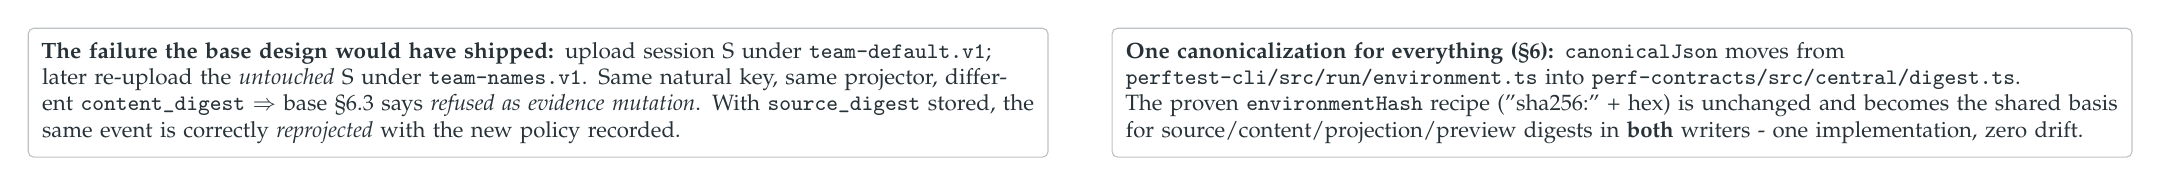
\begin{tikzpicture}[node distance=5mm and 8mm]
\node[note,text width=126mm] (why) {\textbf{The failure the base design would have shipped:} upload session S under \code{team-default.v1}; later re-upload the \emph{untouched} S under \code{team-names.v1}. Same natural key, same projector, different \code{content_digest} $\Rightarrow$ base \S6.3 says \emph{refused as evidence mutation}. With \code{source_digest} stored, the same event is correctly \emph{reprojected} with the new policy recorded.};
\node[note,right=8mm of why,text width=126mm] {\textbf{One canonicalization for everything (\S6):} \code{canonicalJson} moves from \code{perftest-cli/src/run/environment.ts} into \code{perf-contracts/src/central/digest.ts}. The proven \code{environmentHash} recipe ("sha256:" + hex) is unchanged and becomes the shared basis for source/content/projection/preview digests in \textbf{both} writers - one implementation, zero drift.};
\end{tikzpicture}

\end{minipage}
\end{adjustbox}

\newpage
% =====================================================================
% B3. DIAGEVENT MAPPING + RANK LADDER
% =====================================================================
\pagehead{B3. The real \code{DiagEvent} $\to$ row mapping, and the classification ladder}
{C-4/C-5: the envelope is richer than the base table - required eventId, an entity anchor, tags, and a sibling GapRecord stream. \code{cls_rank} has an exact vendorable definition.}
\legend\par\vspace{4mm}

\begin{adjustbox}{max width=\linewidth,max height=0.82\textheight,center}
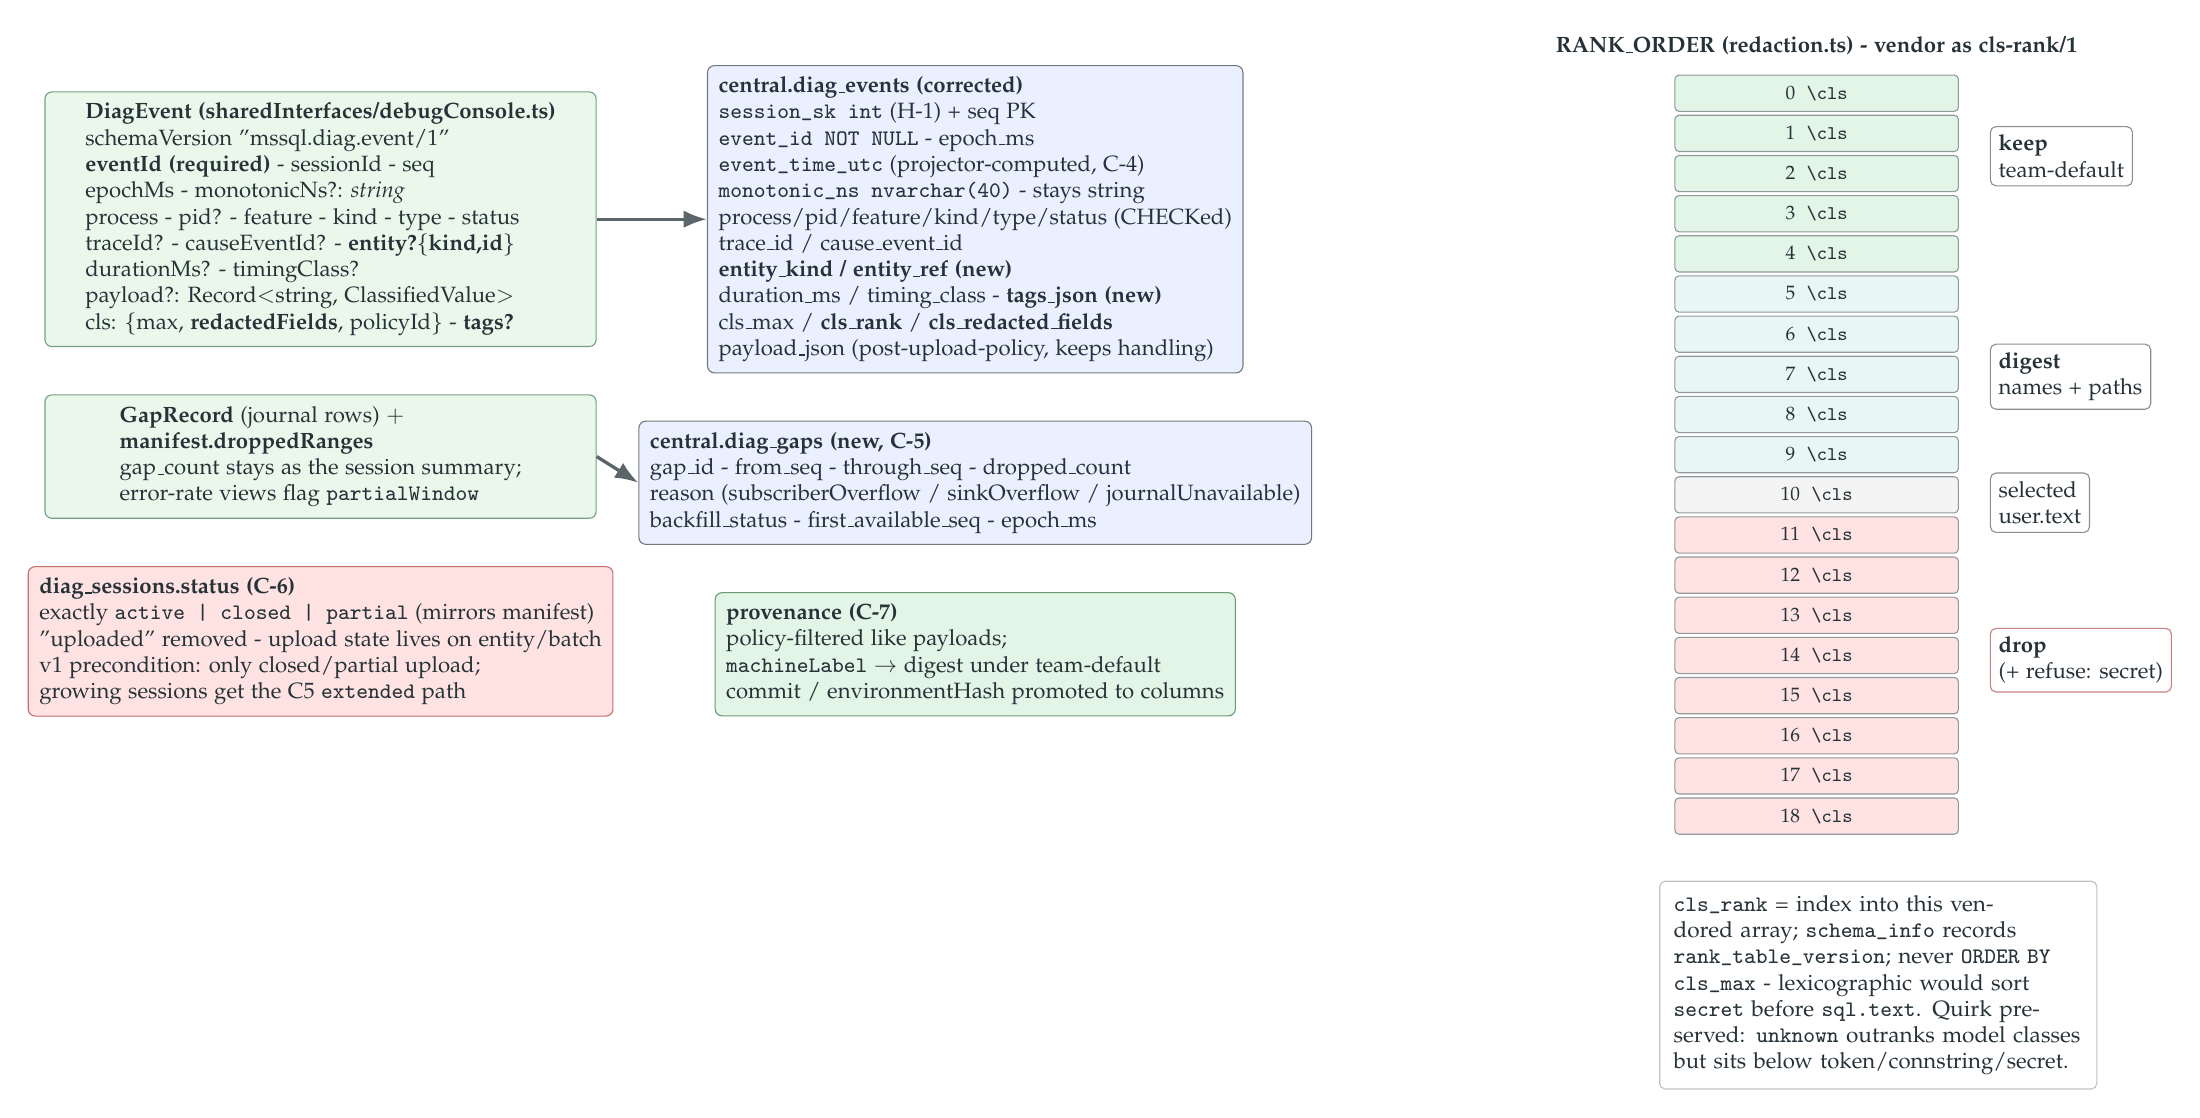
\begin{tikzpicture}[node distance=5mm and 10mm]

% left: envelope -> columns
\node[sourcebox,minimum width=70mm,align=left,font=\footnotesize] (env)
{\textbf{DiagEvent (sharedInterfaces/debugConsole.ts)}\\
schemaVersion "mssql.diag.event/1"\\
\textbf{eventId (required)} - sessionId - seq\\
epochMs - monotonicNs?: \emph{string}\\
process - pid? - feature - kind - type - status\\
traceId? - causeEventId? - \textbf{entity?\{kind,id\}}\\
durationMs? - timingClass?\\
payload?: Record$<$string, ClassifiedValue$>$\\
cls: \{max, \textbf{redactedFields}, policyId\} - \textbf{tags?}};

\node[box,minimum width=66mm,align=left,font=\footnotesize,right=14mm of env] (cols)
{\textbf{central.diag\_events (corrected)}\\
\code{session_sk int} (H-1) + seq PK\\
\code{event_id NOT NULL} - epoch\_ms\\
\code{event_time_utc} (projector-computed, C-4)\\
\code{monotonic_ns nvarchar(40)} - stays string\\
process/pid/feature/kind/type/status (CHECKed)\\
trace\_id / cause\_event\_id\\
\textbf{entity\_kind / entity\_ref (new)}\\
duration\_ms / timing\_class - \textbf{tags\_json (new)}\\
cls\_max / \textbf{cls\_rank} / \textbf{cls\_redacted\_fields}\\
payload\_json (post-upload-policy, keeps handling)};
\draw[arrow] (env.east) -- (cols.west);

\node[box,minimum width=66mm,align=left,font=\footnotesize,below=6mm of cols] (gaps)
{\textbf{central.diag\_gaps (new, C-5)}\\
gap\_id - from\_seq - through\_seq - dropped\_count\\
reason (subscriberOverflow / sinkOverflow / journalUnavailable)\\
backfill\_status - first\_available\_seq - epoch\_ms};
\node[sourcebox,minimum width=70mm,align=left,font=\footnotesize,below=6mm of env] (gsrc)
{\textbf{GapRecord} (journal rows) $+$\\ \textbf{manifest.droppedRanges}\\ \footnotesize gap\_count stays as the session summary;\\ \footnotesize error-rate views flag \code{partialWindow}};
\draw[arrow] (gsrc.east) -- (gaps.west);

\node[riskbox,minimum width=70mm,align=left,font=\footnotesize,below=6mm of gsrc] (sess)
{\textbf{diag\_sessions.status (C-6)}\\ exactly \code{active | closed | partial} (mirrors manifest)\\ "uploaded" removed - upload state lives on entity/batch\\ v1 precondition: only closed/partial upload;\\ growing sessions get the C5 \code{extended} path};
\node[goodbox,minimum width=66mm,align=left,font=\footnotesize,below=6mm of gaps] (prov)
{\textbf{provenance (C-7)}\\ policy-filtered like payloads;\\ \code{machineLabel} $\to$ digest under team-default\\ commit / environmentHash promoted to columns};

% right: rank ladder
\begin{scope}[xshift=172mm,yshift=16mm]
\node[font=\footnotesize\bfseries] at (18mm,6mm) {RANK\_ORDER (redaction.ts) - vendor as cls-rank/1};
\foreach [count=\i from 0] \cls/\band in {public/good, system.metadata/good, diagnostic.metadata/good, result.shape/good, sql.digest/good, source.path/policy, object.name/policy, schema.name/policy, database.name/policy, server.name/policy, user.text/external, sql.text/risk, row.data/risk, model.prompt/risk, model.response/risk, unknown/risk, token/risk, connection.string/risk, secret/risk}{
  \node[draw=ink!50,fill=\band,rounded corners=1.5pt,minimum width=36mm,minimum height=4.6mm,font=\scriptsize,inner sep=1pt] at (18mm,{-\i*5.1mm}) {\i\ \ \code{\cls}};
}
\node[tinybox,anchor=west,align=left] at (40mm,-8mm) {\textbf{keep}\\team-default};
\node[tinybox,anchor=west,align=left] at (40mm,-36mm) {\textbf{digest}\\names + paths};
\node[tinybox,anchor=west,align=left] at (40mm,-52mm) {selected\\user.text};
\node[tinybox,anchor=west,align=left,draw=red!70] at (40mm,-72mm) {\textbf{drop}\\(+ refuse: secret)};
\node[note,text width=52mm,anchor=north west] at (-2mm,-100mm) {\code{cls_rank} = index into this vendored array; \code{schema_info} records \code{rank_table_version}; never \code{ORDER BY cls_max} - lexicographic would sort \code{secret} before \code{sql.text}. Quirk preserved: \code{unknown} outranks model classes but sits below token/connstring/secret.};
\end{scope}

\end{tikzpicture}
\end{adjustbox}

\newpage
% =====================================================================
% B4. PRODUCT WRITER LANE (REAL DATA PLANE)
% =====================================================================
\pagehead{B4. The product writer against the real Data Plane}
{C-11: \code{execute(text, opts, sink)} takes \textbf{no parameters}; commandKind/priority are per-execute. The contract owns the literal encoder, or nothing ships.}
\legend\par\vspace{4mm}

\begin{adjustbox}{max width=\linewidth,max height=0.82\textheight,center}
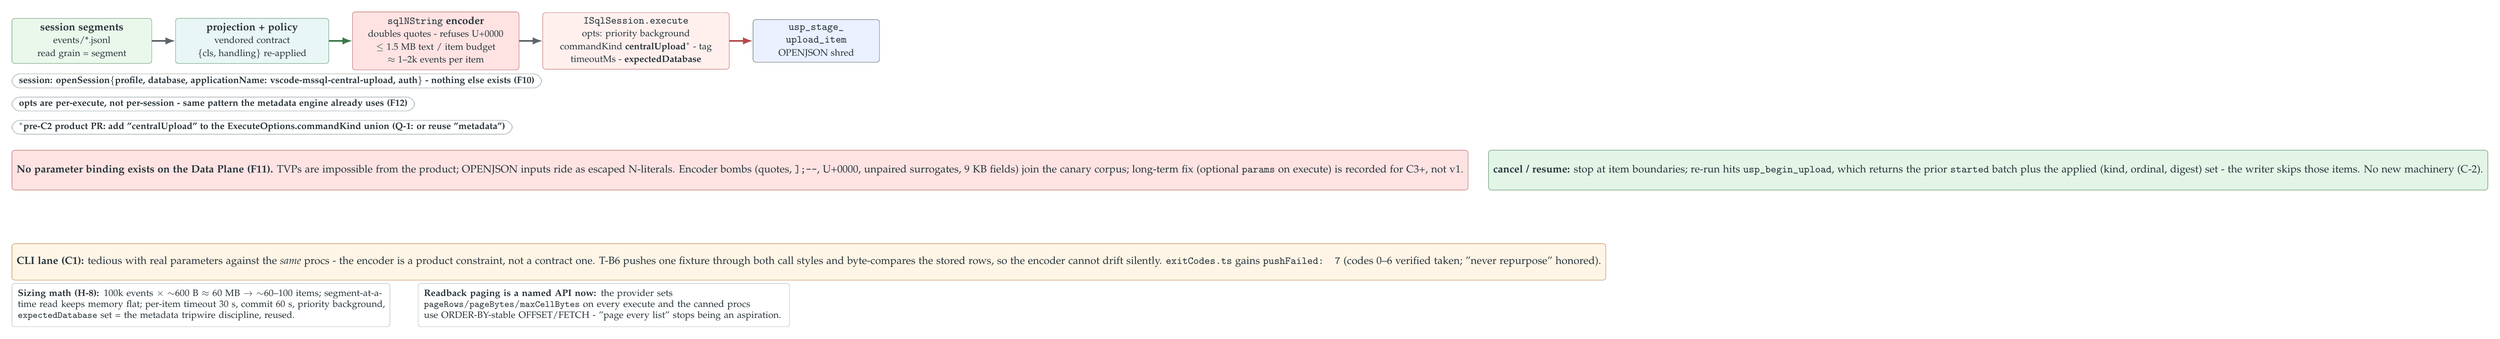
\begin{tikzpicture}[node distance=6mm and 7mm]

\node[sourcebox,minimum width=42mm] (seg) {\textbf{session segments}\\\footnotesize events/*.jsonl\\\footnotesize read grain = segment};
\node[policybox,minimum width=46mm,right=of seg] (projp) {\textbf{projection + policy}\\\footnotesize vendored contract\\\footnotesize \{cls, handling\} re-applied};
\node[riskbox,minimum width=50mm,right=of projp] (enc) {\textbf{\code{sqlNString} encoder}\\\footnotesize doubles quotes - refuses U+0000\\\footnotesize $\le$ 1.5 MB text / item budget\\\footnotesize $\approx$ 1--2k events per item};
\node[writerbox,minimum width=56mm,right=of enc] (exec) {\textbf{\code{ISqlSession.execute}}\\\footnotesize opts: priority background\\\footnotesize commandKind \textbf{centralUpload}$^{*}$ - tag\\\footnotesize timeoutMs - \textbf{expectedDatabase}};
\node[box,minimum width=38mm,right=of exec] (proc) {\textbf{\code{usp_stage_}}\\\textbf{\code{upload_item}}\\\footnotesize OPENJSON shred};
\draw[arrow] (seg) -- (projp);
\draw[policyarr] (projp) -- (enc);
\draw[arrow] (enc) -- (exec);
\draw[write] (exec) -- (proc);

\node[pill,below=3mm of seg.south west,anchor=north west] {session: openSession\{profile, database, applicationName: vscode-mssql-central-upload, auth\} - nothing else exists (F10)};
\node[pill,below=10mm of seg.south west,anchor=north west] {opts are \textbf{per-execute}, not per-session - same pattern the metadata engine already uses (F12)};
\node[pill,below=17mm of seg.south west,anchor=north west] {$^{*}$pre-C2 product PR: add "centralUpload" to the ExecuteOptions.commandKind union (Q-1: or reuse "metadata")};

\node[riskbox,minimum width=120mm,minimum height=12mm,below=26mm of seg.south west,anchor=north west] (nopar)
{\textbf{No parameter binding exists on the Data Plane (F11).} TVPs are impossible from the product; OPENJSON inputs ride as escaped N-literals. Encoder bombs (quotes, \code{];--}, U+0000, unpaired surrogates, 9 KB fields) join the canary corpus; long-term fix (optional \code{params} on execute) is recorded for C3+, not v1.};
\node[goodbox,minimum width=98mm,minimum height=12mm,right=6mm of nopar]
{\textbf{cancel / resume:} stop at item boundaries; re-run hits \code{usp_begin_upload}, which returns the prior \code{started} batch plus the applied (kind, ordinal, digest) set - the writer skips those items. No new machinery (C-2).};

\node[cibox,minimum width=224mm,minimum height=11mm,below=16mm of nopar.south west,anchor=north west]
{\textbf{CLI lane (C1):} tedious with real parameters against the \emph{same} procs - the encoder is a product constraint, not a contract one. T-B6 pushes one fixture through both call styles and byte-compares the stored rows, so the encoder cannot drift silently. \code{exitCodes.ts} gains \code{pushFailed: 7} (codes 0--6 verified taken; "never repurpose" honored).};

\node[note,below=15mm of nopar.south west,anchor=north west,text width=110mm,yshift=-13mm]
{\textbf{Sizing math (H-8):} 100k events $\times$ $\sim$600 B $\approx$ 60 MB $\to$ $\sim$60--100 items; segment-at-a-time read keeps memory flat; per-item timeout 30 s, commit 60 s, priority background, \code{expectedDatabase} set = the metadata tripwire discipline, reused.};
\node[note,right=6mm of {$(nopar.south west)+(116mm,-28mm)$},anchor=north west,text width=108mm]
{\textbf{Readback paging is a named API now:} the provider sets \code{pageRows}/\code{pageBytes}/\code{maxCellBytes} on every execute and the canned procs use ORDER-BY-stable OFFSET/FETCH - "page every list" stops being an aspiration.};

\end{tikzpicture}
\end{adjustbox}

\newpage
% =====================================================================
% B5. PERF TWIN: SUBTRACTIONS + PARITY
% =====================================================================
\pagehead{B5. The perf twin needs a subtraction list, not just additions}
{C-8/C-9/C-10: the local SQLite schema carries paths, machine ids, and free text a naive dialect twin would upload verbatim - and one PK that is illegal in T-SQL.}
\legend\par\vspace{4mm}

\begin{adjustbox}{max width=\linewidth,max height=0.82\textheight,center}
\begin{minipage}{272mm}

\begin{tabular}{p{62mm}p{28mm}p{40mm}p{120mm}}
\toprule
\textbf{local column (perf-store.schema.sql)} & \textbf{class} & \textbf{team-default / ci} & \textbf{central rule} \\
\midrule
runs.output\_dir - runs.config\_path - repetitions.result\_path & source.path & \cellcolor{risk}\textbf{drop} & absolute local paths never cross the boundary \\
runs.machine\_id - environments.machine\_id & label & \cellcolor{policy}digest & plain label only under team-names \\
runs.notes - baselines.notes & user.text & \cellcolor{risk}\textbf{drop} & keep under team-names+ \\
artifacts.path & source.path & \cellcolor{policy}relative-only & projection verifies relative to run root; absolute $\Rightarrow$ refusedByPolicy (Q-3) \\
baselines.created\_by & user label & \cellcolor{policy}$\to$ uploader\_id FK & no free-text principals centrally \\
environments.* (os/cpu/mem/versions), config\_fingerprint\_json, sql\_image\_digest & system.metadata & \cellcolor{good}keep & the join keys the feature exists for \\
metrics.* - validations.* - repetitions ids/status/warmup/trace/*\_unix\_ns & diagnostic.metadata & \cellcolor{good}keep & unix-ns strings persist as truth + projector-computed *\_utc for indexing \\
comparisons.* - comparison\_metrics.* & derived & \cellcolor{external}local-only & central recomputes trends via views (Q-7) \\
\bottomrule
\end{tabular}

\vspace{5mm}
\begin{tikzpicture}[node distance=6mm and 8mm]
\node[goodbox,minimum width=88mm,align=left,font=\footnotesize] (att)
{\textbf{attempt\_id is real (C-9)}\\ repetitions and metrics carry \code{attempt_id INTEGER NOT NULL DEFAULT 0};\\ the central twin adds it to repetitions, metrics, validations, artifact\_refs.};
\node[policybox,minimum width=104mm,align=left,font=\footnotesize,right=of att] (parity)
{\textbf{official\_metric\_samples parity surface (frozen)}\\ join \code{(run_id, scenario_id, rep_id, attempt_id)};\\ \code{WHERE m.official=1 AND r.pass_type='measurement' AND rep.status='passed'}\\ - reproduced exactly; central extras go in \code{official_metric_samples_ex}. T-B7 byte-compares fixture rows across engines.};
\node[riskbox,minimum width=70mm,align=left,font=\footnotesize,right=of parity] (pk)
{\textbf{baselines PK is illegal as twinned (C-10)}\\ SQLite allows NULL inside the composite PK; T-SQL does not.\\ Central: surrogate \code{baseline_id} + \code{UNIQUE} with \code{''} wildcard sentinels; codec documents NULL $\leftrightarrow$ \code{''}; writes only via role-gated \code{usp_set_baseline}.};
\end{tikzpicture}

\vspace{4mm}

\begin{tikzpicture}
\node[pill] (p1) {runs.status centrally includes 'aborted' (present locally, missing from base prose)};
\node[pill,right=6mm of p1] (p2) {every kind table += upload\_batch\_id NOT NULL (C-3)};
\node[pill,right=6mm of p2] {goldens embody this map - conformance is byte-level (T-B5)};
\end{tikzpicture}

\end{minipage}
\end{adjustbox}

\newpage
% =====================================================================
% B6. READER STATES, RETENTION, PURGE
% =====================================================================
\pagehead{B6. Honest reader states, retention lanes, and purge}
{C-12 + H-1/H-4: the state ladder is a real union extension in \code{perfHistory.ts}; filtered-ness is a query-result fact; retention deletes whole sessions.}
\legend\par\vspace{4mm}

\begin{adjustbox}{max width=\linewidth,max height=0.82\textheight,center}
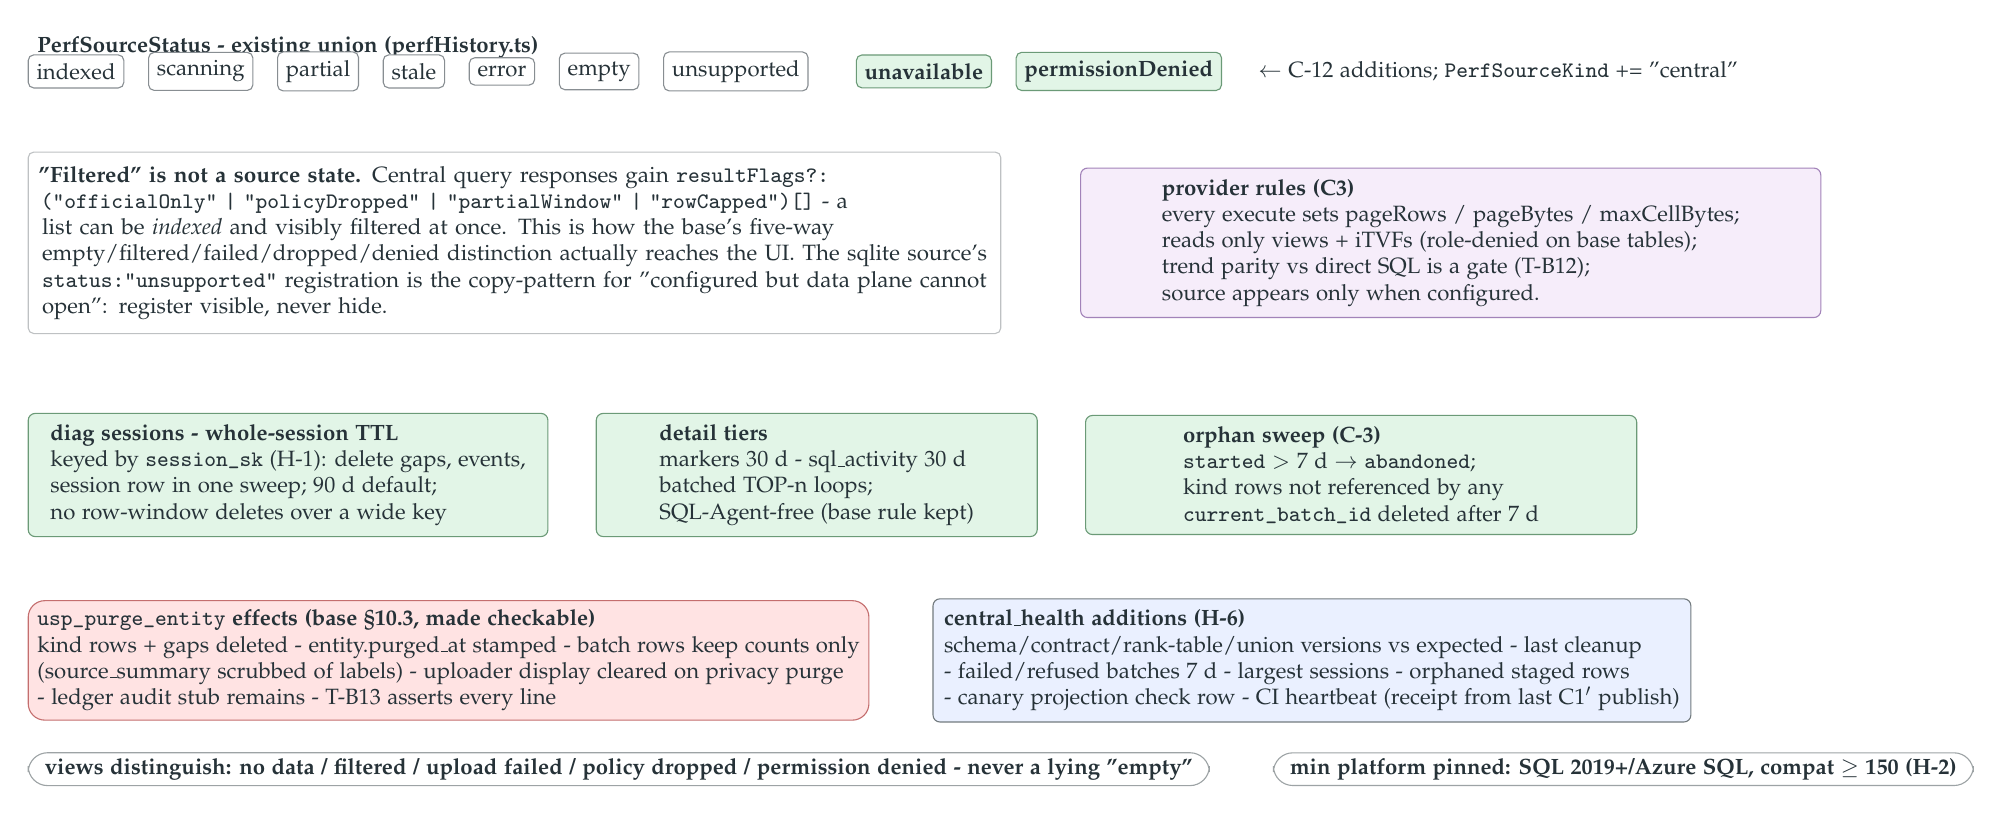
\begin{tikzpicture}[node distance=5mm and 6mm]

% union extension
\node[font=\footnotesize\bfseries] (t1) {PerfSourceStatus - existing union (perfHistory.ts)};
\node[tinybox,below=3mm of t1.west,anchor=west] (s1) {indexed};
\node[tinybox,right=3mm of s1] (s2) {scanning};
\node[tinybox,right=3mm of s2] (s3) {partial};
\node[tinybox,right=3mm of s3] (s4) {stale};
\node[tinybox,right=3mm of s4] (s5) {error};
\node[tinybox,right=3mm of s5] (s6) {empty};
\node[tinybox,right=3mm of s6] (s7) {unsupported};
\node[tinybox,right=6mm of s7,fill=good,draw=green!75] (s8) {\textbf{unavailable}};
\node[tinybox,right=3mm of s8,fill=good,draw=green!75] (s9) {\textbf{permissionDenied}};
\node[label,right=4mm of s9] {$\leftarrow$ C-12 additions; \code{PerfSourceKind} += "central"};

\node[note,below=8mm of s1.south west,anchor=north west,text width=120mm] (flags)
{\textbf{"Filtered" is not a source state.} Central query responses gain \code{resultFlags?: ("officialOnly" | "policyDropped" | "partialWindow" | "rowCapped")[]} - a list can be \emph{indexed} and visibly filtered at once. This is how the base's five-way empty/filtered/failed/dropped/denied distinction actually reaches the UI. The sqlite source's \code{status:"unsupported"} registration is the copy-pattern for "configured but data plane cannot open": register visible, never hide.};

\node[readerbox,minimum width=94mm,align=left,font=\footnotesize,right=10mm of flags] (prov)
{\textbf{provider rules (C3)}\\ every execute sets pageRows / pageBytes / maxCellBytes;\\ reads only views + iTVFs (role-denied on base tables);\\ trend parity vs direct SQL is a gate (T-B12);\\ source appears only when configured.};

% retention lanes
\node[goodbox,minimum width=66mm,align=left,font=\footnotesize,below=10mm of flags.south west,anchor=north west] (r1)
{\textbf{diag sessions - whole-session TTL}\\ keyed by \code{session_sk} (H-1): delete gaps, events,\\ session row in one sweep; 90 d default;\\ no row-window deletes over a wide key};
\node[goodbox,minimum width=56mm,align=left,font=\footnotesize,right=6mm of r1] (r2)
{\textbf{detail tiers}\\ markers 30 d - sql\_activity 30 d\\ batched TOP-n loops;\\ SQL-Agent-free (base rule kept)};
\node[goodbox,minimum width=70mm,align=left,font=\footnotesize,right=6mm of r2] (r3)
{\textbf{orphan sweep (C-3)}\\ \code{started} $>$ 7 d $\to$ \code{abandoned};\\ kind rows not referenced by any\\ \code{current_batch_id} deleted after 7 d};

\node[badstate,minimum width=96mm,align=left,font=\footnotesize,below=8mm of r1.south west,anchor=north west,minimum height=15mm] (purge)
{\textbf{\code{usp_purge_entity} effects (base \S10.3, made checkable)}\\ kind rows + gaps deleted - entity.purged\_at stamped - batch rows keep counts only\\ (source\_summary scrubbed of labels) - uploader display cleared on privacy purge\\ - ledger audit stub remains - T-B13 asserts every line};
\node[box,minimum width=96mm,align=left,font=\footnotesize,right=8mm of purge,minimum height=15mm] (health)
{\textbf{central\_health additions (H-6)}\\ schema/contract/rank-table/union versions vs expected - last cleanup\\ - failed/refused batches 7 d - largest sessions - orphaned staged rows\\ - canary projection check row - CI heartbeat (receipt from last C1$'$ publish)};

\node[pill,below=4mm of purge.south west,anchor=north west] (bp1) {views distinguish: no data / filtered / upload failed / policy dropped / permission denied - never a lying "empty"};
\node[pill,right=8mm of bp1] {min platform pinned: SQL 2019+/Azure SQL, compat $\ge$ 150 (H-2)};

\end{tikzpicture}
\end{adjustbox}

\end{document}
